
\section{Benchmark Model} \label{Benchmark}

As discussed in Section \ref{Problem}, SK has already performed a search for the mode we are studying here. This particular mode is sometimes called prompt-gamma method, since it relies on the coincidence measurement of the muon and the photon that is promptly emitted by the nucleus. The details of the analysis, as well as the final results can be found in \cite{Miura}, but figure \ref{fig:benchmark} shows a table that summarizes the main results of that search.

\begin{figure}[h]
  \centering
  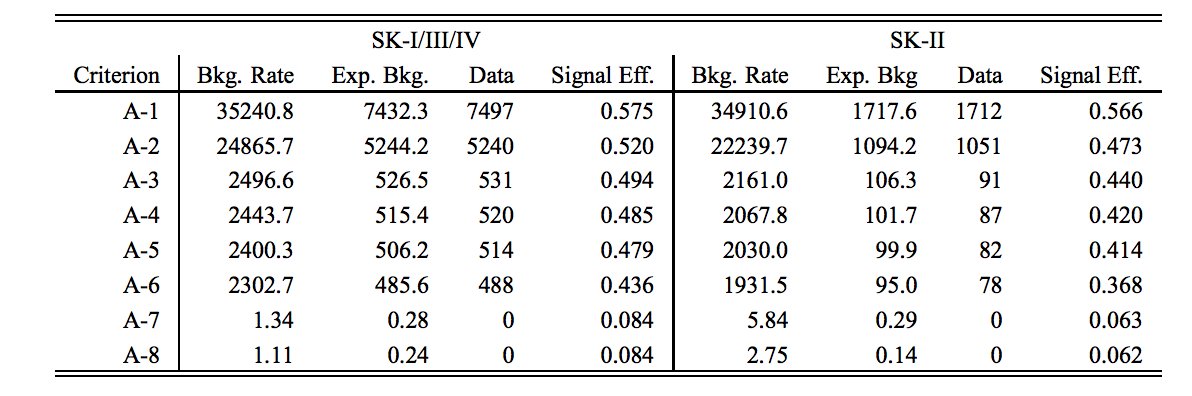
\includegraphics[width=0.8\linewidth]{figs/benchmark.png}
  \caption{Summary of the results obtained in the standard analysis done in SK. Definition of all quantities is given in the text.}
  \label{fig:benchmark}
\end{figure}

The criteria A1-8 are the different cuts applied in that analysis, the background rate is explained in more detail in Section \ref{Background}, eq. \ref{eq:mtonyear}, but basically it refers to the expected number of false positives if the detector had 1 million tones of volume and took data for 1 year. The expected background is the number of false positives in the analyzed data after each cut $\textrm{A}-i$ is applied, and the Data column corresponds to the actual number observed. 
Finally, the Signal Efficiency is defined in eq. \ref{eq:eff} in Section \ref{Efficiency} and corresponds to recall, i.e., the probability that an event is classified as signal given that it is signal.

The table contains values for all SK eras, from I to IV. SK-II is different due to an accident that reduced the number of PMTs, so the photo-coverage is different. We are using simulated data for SK-IV only, while the table contains the averaged results of SK I, III and IV. SK-IV performance if better than I and III due to better electronics and other factors,  but since the performance is not super different. We can use the numbers in the first column as our benchmark model.

The efficiency in the last column is reported to be 

\begin{equation} \label{eq:effB}
\epsilon_{B} = 0.084 = 8.4\%,
\end{equation}

where $B$ stands for Benchmark. This is one of the main numbers we wanna compare to, so using the definition of efficiency given in \ref{eq:eff} and the necessary scale factor discussed in Section \ref{Efficiency}, we can make a comparison between all classifiers used in this study and the benchmark model.

Also, since the amount of data analyzed will be different, we have to compare the number of false positives in our analysis with the $\textrm{Mton}\cdot\textrm{year}$ rate provided in the table. Section \ref{Background} explain the necessary transformations we need to do with FP to compare with the benchmark rate. Eq. \ref{eq:mtonyear} gives the rescale for our analysis and the benchmark result we can define as:

\begin{equation} \label{eq:MtonB}
R_{B} = 1.1\textrm{ event per Mega-tone per year}.
\end{equation}

Section \ref{Metric} discusses different metrics that will be used in this study. They will be useful when comparing different classifiers among themselves, but to compare our final results with the benchmark model provided by the standard analysis of SK, I will use the efficiency and rate defined here in eqs. \ref{eq:effB} and \ref{eq:MtonB}.

